\chapter{Distilling structural and contextual qualities of document
embeddings}\label{chapter:training_method}

In this chapter, we introduce our method of training document embeddings. We
base our approach on teacher-student training, distilling the knowledge of two
embedding models (referred to as \emph{teachers}) into one  \emph{student}
model. Section~\ref{section:training_method} explains our training method in
detail and outlines the used loss function. In the rest of this chapter, we
describe the two teacher models in Section~\ref{section:teacher_models} and the
student in Section~\ref{section:student_model}.

\section{Training methodology}\label{section:training_method}

Our training methodology aims to train an embedding model such that its
embeddings more faithfully represent the input. As we describe in
Chapter~\ref{chapter:document_representation}, we distinguish two qualities of
faithful representations: structural and contextual. The goal is to instill
both qualities into a single embedding model. To do so, we use teacher-student
training with two teacher embedding models, one with high structural capacity
and the other with high contextual capacity.

In the following subsections, we describe teacher-student training in detail
and give a high-level overview of the proposed loss function.

\subsection{Teacher-student training}

In the teacher-student training, we train a student model based on a frozen
teacher model. The goal is to make the student model imitate the teacher model,
thereby digesting the teacher's understanding of the input. Although the
student model is generally not expected to outperform the teacher model,
teacher-student training is still valuable in several situations. For instance,
\cite{sanh2019distilbert} use teacher-student training to make a model smaller
while sacrificing only a fraction of its performance. In another scenario,
\cite{reimers2020making} use teacher-student training to enforce similarity
between models' outputs, thereby giving the student model a powerful training
signal.

We assume two embedding models in our setting: a structural teacher
$\Teacher_S$ and a contextual teacher $\Teacher_C$ with high structural and
contextual capacities, respectively. Teacher-student training allows us to
instill both capacities into a third student model {\Student} while avoiding
the architectural limitations of the teachers. We hypothesize that we can
efficiently direct the two training signals so that they do not push against
each other.


\subsection{Abstract loss formulation}\label{section:abstract_loss}


We instill a quality of a teacher's embedding by simply enforcing a similarity
between the teacher's and student's embedding. Since we have two teachers, we
use two similarities $\Loss_S$, and $\Loss_C$, which compare the student's
embedding $y_\Student$ with the structural teacher's embedding $y_{\Teacher_S}$
and the contextual teacher's embedding $y_{\Teacher_C}$, respectively. We show
a graphical overview of the training architecture in
Figure~\ref{fig:teacher_student_train_arch}.

To regulate the mixture of $\Loss_S$ and $\Loss_C$, we introduce weighting
parameter $\lambda$. In the most general form, we assume $\lambda$ to be
dependent on the input text $x$ since the performance of the teacher models
might vary across different inputs. In particular, we can expect $\lambda$ to
depend on the length of the input since, for shorter inputs, the context
is minimal and, therefore, expendable. Abstract formulation of the loss is
given in Equation~\ref{eq:abstract_loss}. We explore concrete options for
$\Loss_S$, $\Loss_C$ and $\lambda(x)$ in Chapter~\ref{chapter:experiments}.

\begin{equation}\label{eq:abstract_loss}
  \Loss(
    x,
    y_\Student,
    y_{\Teacher_S},
    y_{\Teacher_C},
    \lambda
  ) =
    \lambda(x) \Loss_S(y_\Student, y_{\Teacher_S}) +
            (1 - \lambda(x)) \Loss_C(y_\Student, y_{\Teacher_S})
\end{equation}

The two losses could push against each other and slow down or halt the
training. To avoid that, we choose one of the losses to be more strict while
the other to be more forgiving. In that way, the more forgiving loss should
adapt to the strict one instead of pushing against it. As mentioned in
Section~\ref{section:combine_structural_and_contextual}, we view structural
quality as the more important. Therefore, we choose the structural loss
$\Loss_S$ as the stricter and exact loss, forcing the student to mimic the
structural teacher as much as possible. On the other hand, the contextual loss
$\Loss_C$ should give the student model more freedom in the form of the
produced embedding but still force it to incorporate the information from the
contextual embedding.

\begin{figure}
  \centering
  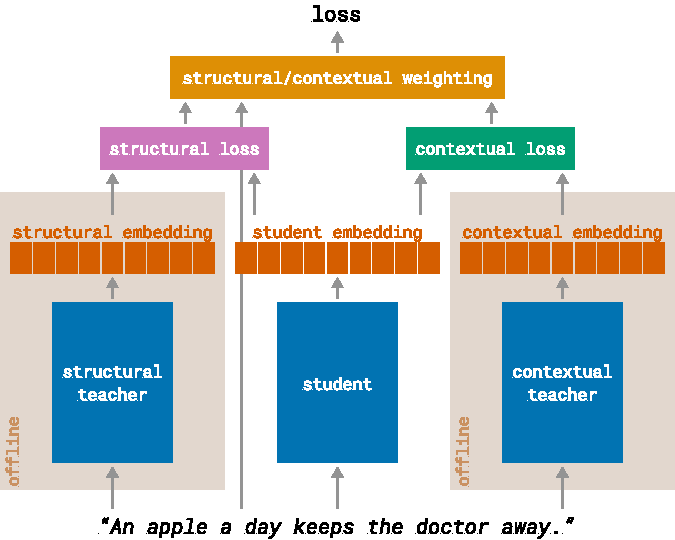
\includegraphics[width=0.8\textwidth]{./img/training_architecture.pdf}

  \caption{The architecture of our teacher-student training. We distill the
  qualities of the teachers' embeddings through corresponding losses into a
  student model. Since we do not update the weights of either teacher,
  the generation of their embeddings can be done offline before training.}

  \label{fig:teacher_student_train_arch}

\end{figure}

\section{Teacher models}\label{section:teacher_models}

This section introduces the teacher models used during our experiments in
Chapter~\ref{chapter:experiments}. We chose Sentence-BERT
\citep{reimers2019sentence} as the structural teacher model and Paragraph
Vector \citep{le2014distributed} (or \emph{PV}) as the context teacher model.
As explained in Chapter~\ref{chapter:document_representation}, each of the two
mentioned models specializes in a different quality of produced embeddings.
SBERT can compare word relationships on many levels and thus understand even
complex text structures. However, it cannot process long texts. On the other
hand, Paragraph Vectors can produce embeddings even for long documents, but they
process text very shallowly, which prohibits understanding any complex
structures. We hope to synthesize both qualities by combining the two
teacher models in a single model.

\subsection{SBERT}

Sentence-BERT is a composition of a BERT-like \citep{devlin2019bert} encoder
with a mean pooling layer above its last layer's hidden states. The model is
finetuned with Natural Language Inference (\emph{NLI}) datasets to produce
semantically meaningful embeddings. We illustrate SBERT's training
architecture in Figure~\ref{fig:sbert}. We have chosen SBERT as a structural
teacher for its high structural capacity and strong performance in
sentence-level text-understanding tasks \citep{reimers2019sentence}.

\begin{figure}
  \centering
  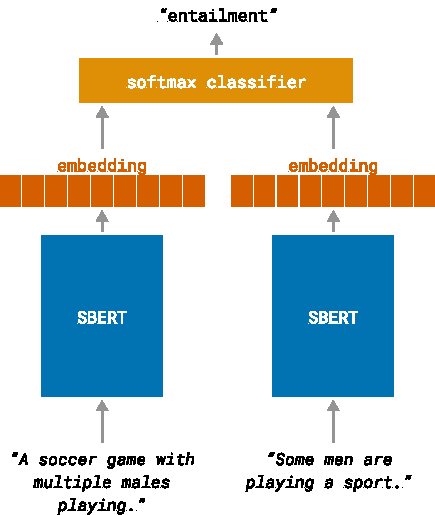
\includegraphics[width=0.5\textwidth]{./img/sbert_architecture.pdf}

  \caption{Siamese network architecture used to train SBERT. The pair of
  sentences from an NLI dataset is classified into three classes
  ``entailment'', ``neutral'' and ``contradiction''.}

  \label{fig:sbert}

\end{figure}

\subsection{Paragraph Vector}\label{section:paragraph_vector}

Paragraph Vector \citep{le2014distributed}, sometimes referred to as Doc2Vec, is a simple
text-embedding model that views the input as a Bag of Words (or BoW). Paragraph
Vector comprises two sub-models: Distributed Memory (DM) and Distributed Bag of
Words (DBOW). While each model is trained separately, the authors recommend combining both architectures into a single model, where the combined models' embeddings are simply concatenated. The models are trained to
predict a word within a window in the given document. As shown in
Figure~\ref{fig:dbow}, DBOW bases its prediction only on the whole paragraph's embedding. On the other hand, DM, whose architecture is depicted in
Figure~\ref{fig:dm}, additionally uses the embeddings of the surrounding words
within a given window.

We chose Paragraph Vector as a contextual teacher due to its unique
architecture, which forces the model to develop a single vector that summarizes
the common theme of the document. Moreover, Paragraph Vector does not have a
limited maximum input length, so as a contextual teacher, it will always
provide some signal to the student regarding the document's context. Also, even
though Paragraph Vector cannot match the performance of substantially more
complex models such as Transformers, \cite{dai2015document} show that for
larger datasets, Paragraph Vector, outperforms classical embedding models such
as Latent Dirichlet Allocation \citep{blei2003latent} or TF-IDF weighted BoW
model \citep{harris1954distributional}. Finally, Paragraph Vector's simple
architecture allows it to train on significantly larger text corpora than other
bigger models, such as SBERT. Therefore, for a given computational budget,
Paragraph Vector would see more documents during training than SBERT, which may
give it a slight advantage.

\begin{figure}
  \centering
  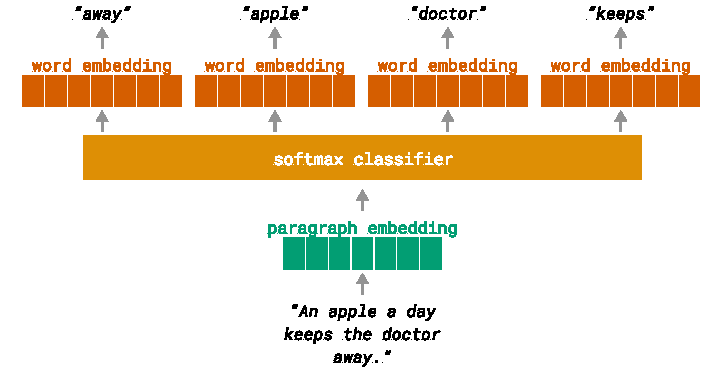
\includegraphics[width=0.8\textwidth]{./img/dbow_architecture.pdf}

  \caption{Architecture of Distributed Bag of Words. The model predicts words
  from a document, only using the document's embedding.}

  \label{fig:dbow}
\end{figure}

\begin{figure}
  \centering
  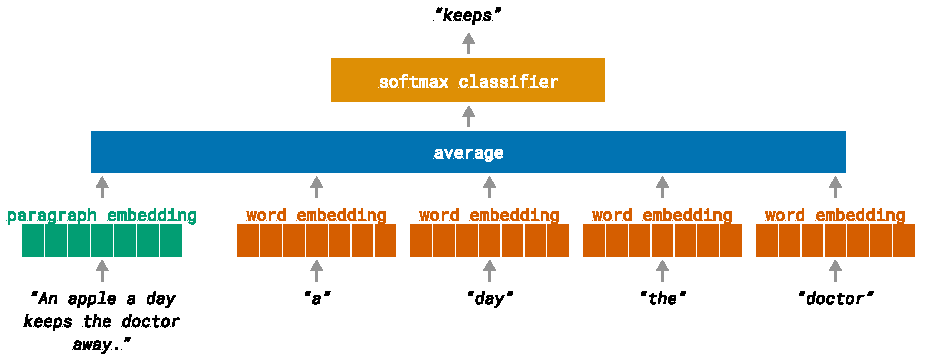
\includegraphics[width=1\textwidth]{./img/dm_architecture.pdf}

  \caption{Distributed Memory model architecture. The model predicts the input
  words' neighboring word for the input paragraph.}

  \label{fig:dm}

\end{figure}

\section{Student model}\label{section:student_model}

In our teacher-student training, the student model is our primary embedding
model, which we train based on the outputs of the teacher models. By using
teacher-student training, we can avoid some of the architectural drawbacks of
both teacher models while still benefiting from the qualities of the teachers'
embeddings. We choose the student's architecture at a midpoint between
the two teachers' architectures. In other words, not to be as complex as the
architecture of SBERT, so it can process longer inputs while still having a
manageable memory footprint, but not as simple as the architecture of PV, so
that the student can model complex world relationships. We chose a Transformer
with a sparse attention mechanism. Transformer is a well-tested architecture
that is used throughout NLP. Additionally, with sparse attention, Transformers
consume a relatively small amount of memory even for longer inputs, as we
explain in Section~\ref{section:efficient_self_attn}. Another consideration is
that we need a pre-trained model, as our method is not suited to train a model
from scratch but to finetune a model's document embeddings.

Contrary to the selection of architecture, selecting a concrete model is not
crucial to our method. Our choice of the concrete model is governed more by
practical considerations rather than the conditions of our method. Since we
have limited computational resources, we prefer a smaller model that we can fit
on a consumer-grade GPU card. We also value the model's performance, ease of
use, and simplicity. We choose Longformer \citep{beltagy2020longformer} as it
is reasonably small, memory efficient, performs above average compared to other
similar models \citep{tay2020long}, and its self-attention mechanism is
straightforward. Other alternatives are BigBird \citep{zaheer2020big}, or if we
would not mind a more complex model, we could use Reformer
\citep{kitaev2020reformer}, Linformer \citep{wang2020linformer} or Performer
\citep{choromanski2020rethinking}.

\subsection{Longformer}

Longformer \citep{beltagy2020longformer} is a Transformer encoder with sparse
attention. Because we refer to Longformer's configuration and training in the
following chapters, we briefly explain Longformer's self-attention mechanism
and the training data of the pre-trained checkpoint.


\subsubsection{Self-attention mechanism}

Longformer has a sparse self-attention mechanism that composes three different
patterns: local, global, and dilated local attention. Local attention is simply
full attention but only within the neighborhood of $\frac{1}{2}\omega$ tokens
on either side of the key token. $\omega$ can be set differently per
self-attention layer. In global attention, few selected tokens attend to all
other tokens. The tokens on which Longformer computes global attention can be
selected per each input. Global attention's parameters are not pre-trained.
Instead, at the beginning of the training, they are initialized by the
parameters from local attention and finetuned for a given task. With dilated
local attention, every key token attends to every $k$ neighboring query token.
So, it is analogous to a one-dimensional Convolution layer
\citep{van2016wavenet} with stride, or dilatation of $k$. However, to use
dilated local attention, one has to use a custom CUDA kernel or a slow
implementation in Python using loops. The authors also provide a reasonably
fast, memory-efficient block implementation for global and local
attention.

\subsubsection{Training}

Longformer is warm-started from a RoBERTa \citep{liu2019roberta} checkpoint
with its learned positional embeddings duplicated eight times to support inputs
up to 4096 tokens long. The authors show that duplicating RoBERTa's positional
embeddings is faster than training position embeddings for all 4096 positions
from scratch. Then, the authors train Longformer using MLM on long documents
for 65k gradient steps to improve its capabilities for longer inputs. The
training corpus overlaps with RoBERTa's pretraining corpus but is more focused
on longer pieces of text. It includes the following datasets:

\begin{itemize}

  \item Book corpus \citep{zhu2015aligning}

  \item English Wikipedia

  \item One-third of articles from Realnews dataset \citep{zellers2019defending}
      with more than 1200 tokens

  \item One-third of the Stories corpus \citep{trinh2018simple}

\end{itemize}

Unfortunately, as of this writing, the Book corpus is unavailable due to
licensing issues. Moreover, we have not been able to find a comparable
alternative. The Stories corpus is also unavailable. However, there is an
alternative\footnote{\url{https://huggingface.co/datasets/spacemanidol/cc-stories}}
that tries to mimic the dataset from the original paper.
